% ---------------------------------------------------------------------------
\section{Post-Deployment Monitoring}
\label{sec:monitoring}
% ---------------------------------------------------------------------------

\subsection{A temporal replay}

The competition's unlabelled file carries no prices, so it cannot support performance
monitoring: drift can be measured, but realised error cannot. The project therefore
builds a genuine replay. The reference model is the selected estimator refitted on the
945 sales completed before January 2009, the vintage that would have been in
production then; its out-of-fold root mean squared error is 20,888 \USD{} and its
MAPE 7.88 per cent. The stream is the 513 sales completed between January 2009 and
July 2010, split into four equal-volume windows of 128 or 129 transactions. Realised prices are treated as
labels that arrive only after a window closes, mirroring the delay between listing
activity and recorded deeds. The design has the property that matters: the monitoring
period is strictly outside the reference model's training data, so accuracy and
coverage measured on the stream are honest out-of-sample quantities. It also has a
limitation that must be stated: the stream is a replayed history, so the monitoring
layer is exercised against a realistic sequence of sales but not against the
operational failures, such as late or duplicated data, that a production feed would
present.

\subsection{What is monitored}

Four families of signal are tracked. Input drift is measured for numeric features by
the population stability index (PSI) on ten reference quantiles, with the
Kolmogorov--Smirnov statistic as a distribution-free cross-check; categorical drift
uses PSI on level proportions with total variation distance; prediction drift is the
PSI of the score distribution, which captures the shift users would notice; and
realised performance is measured by rolling RMSE, MAE, MAPE, mean signed bias, the
business tolerance rate and the empirical coverage of both intervals. PSI is
interpreted with the conventional bands: below 0.10 stable, 0.10 to 0.20 moderate and
0.20 or above significant \citep{siddiqi2006,yurdakul2018psi}. Because the index sums
weighted divergences over bins, empty bins are floored at $10^{-4}$ and the outer
edges are widened to infinity, which prevents a single unseen value from producing an
unbounded index.

\subsection{Window-level results}

Table~\ref{tab:monitoring-windows} reports the observed replay. Accuracy degrades
modestly: root mean squared error rises from 22,306 \USD{} in the first two windows to
23,395 \USD{} in the third and 21,839 \USD{} in the fourth, which corresponds to RMSE
ratios of 1.068, 1.068, 1.120 and 1.046 against the reference. No window crosses the
1.2 ratio that would trigger the accuracy rule, and mean absolute percentage error
stays between 9.14 and 9.63 per cent.

\begin{table}[htbp]
\centering
\caption{Observed replay of the 2009--2010 stream through four equal-volume
chronological windows. The reference model was fitted on 945 sales from January 2006
to December 2008 (out-of-fold RMSE 20,888 \USD).}
\label{tab:monitoring-windows}
\small
\begin{tabular}{@{}lrrrrrr@{}}
\toprule
\textbf{Window} & \textbf{Sales} & \textbf{RMSE} & \textbf{MAE} & \textbf{MAPE} & \textbf{Bias} & \textbf{90\%} \\
 & & (\USD) & (\USD) & (\%) & (\%) & \textbf{coverage} \\
\midrule
W1, 2009-01 to 2009-06 & 129 & 22,306 & 14,813 & 9.41 & $-0.16$ & 0.891 \\
W2, 2009-06 to 2009-09 & 128 & 22,306 & 16,143 & 9.14 & $-1.57$ & 0.875 \\
W3, 2009-09 to 2010-04 & 128 & 23,395 & 15,977 & 9.63 & $-2.52$ & 0.836 \\
W4, 2010-04 to 2010-07 & 128 & 21,839 & 16,048 & 9.34 & $-4.99$ & 0.797 \\
\bottomrule
\end{tabular}
\end{table}

Calibration behaves very differently from accuracy. The 90 per cent interval covers
89.1 per cent of sales in the first window, 87.5 in the second, 83.6 in the third and
79.7 in the fourth; the 80 per cent interval falls from 76.7 to 65.6 per cent over the
same sequence. The intervals are not becoming wider or narrower in any material way;
the distribution of realised prices is moving away from the calibrated residuals.
This is the failure mode that a point-estimate dashboard would miss entirely, and it
is the strongest argument for monitoring calibration alongside accuracy.

\subsection{Drift}

Figure~\ref{fig:drift} shows the PSI by window for twelve informative features and
for the prediction distribution, alongside the window-level performance in
Table~\ref{tab:monitoring-windows}.
Between five and seven of the 43 monitored features exceed the 0.20 threshold in every
window, and the same block is responsible each time: mortgage rate, house price index,
its year-on-year change, local unemployment and months of supply. This is precisely
the block simulated to follow the 2006--2011 cycle, and the reference vintage ends in
December 2008, so the stream contains the steepest part of the rate decline and the
bottom of the price index. The model has no comparable observations in its training
window, which is why both the PSI and the coverage respond.

\begin{figure}[htbp]
\centering
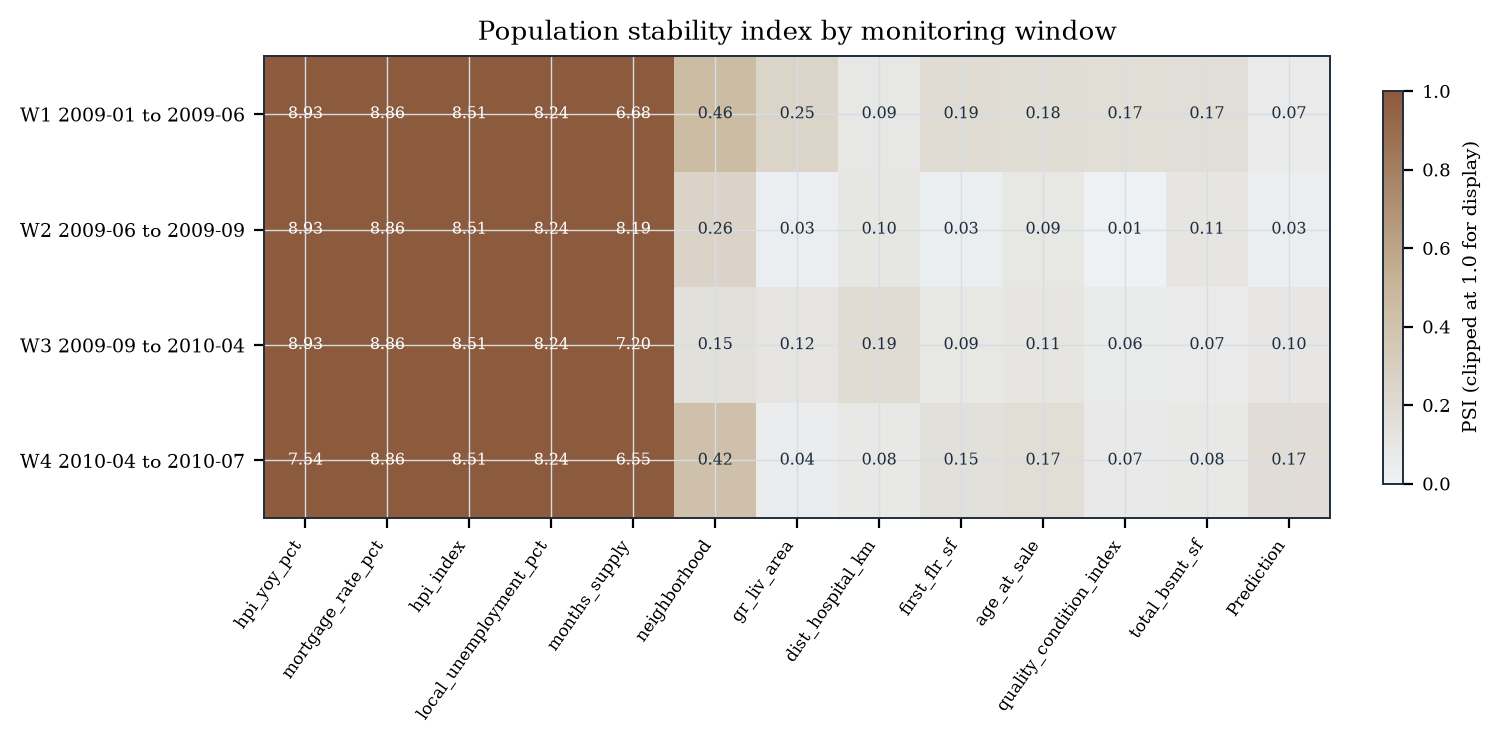
\includegraphics[width=\linewidth]{fig22_drift_heatmap.png}
\caption{Population stability index by monitoring window for the most informative
features and for the prediction distribution. Values are clipped at 1.0 for display;
the untruncated macro values reach 8.9 because the reference window contains almost
none of the later rate and index levels.}
\label{fig:drift}
\end{figure}

Two details deserve interpretation. The neighbourhood indicator also drifts, with a
PSI of 0.46 in the first window and 0.42 in the fourth, because the mix of
neighbourhoods sold changes between periods: a moderate compositional change that a
platform would investigate before concluding that the market itself had moved.
Second, prediction drift rises from 0.066 to 0.174, moderate rather than significant,
even though input drift on the macro block is extreme, because that block carries only
1.14 per cent of in-sample attribution. Prediction drift alone would have understated
the problem; it is the combination of drift, coverage and bias that identifies the
failure.


\subsection{Alert rules and the retraining decision}

Nine rules are evaluated on every run, grouped into input drift, prediction drift,
accuracy, coverage and bias, with sustained versions of the accuracy, coverage and
bias rules elevated to critical severity (Table~\ref{tab:rules}). The observed replay
raises four R1 warnings, two R4 coverage warnings and one critical R7 alert for
sustained coverage erosion. R5 does not fire, because the final-window bias of $-4.99$
per cent sits just inside the 5 per cent threshold, and the accuracy rules do not
fire because no window exceeds 1.2 times the reference RMSE.

\begin{table}[htbp]
\centering
\caption{Monitoring and retraining policy. A critical alert opens a retraining
ticket. The observed replay triggers R1, R4 and R7; the stress scenario additionally
triggers R5.}
\label{tab:rules}
\small
\begin{tabularx}{\linewidth}{@{}L{0.05\linewidth}L{0.31\linewidth}L{0.10\linewidth}X@{}}
\toprule
\textbf{Rule} & \textbf{Condition} & \textbf{Severity} & \textbf{Action} \\
\midrule
R1 & At least 3 features with PSI $\geq$ 0.20 & Warning & Review input pipeline and market context \\
R2 & Prediction PSI $\geq$ 0.20 & Warning & Confirm shift is explained by market moves \\
R3 & Window RMSE $>$ 1.2 $\times$ reference & Critical & Inspect worst errors, prepare retraining \\
R4 & 90\% coverage $<$ 0.85 & Warning & Recalibrate conformal quantiles \\
R5 & $|$mean signed bias$|$ $>$ 5\% & Warning & Verify the macro feed and sale dates \\
R6 & R3 in two consecutive windows & Critical & Retrain \\
R7 & R4 in two consecutive windows & Critical & Recalibrate and retrain if erosion persists \\
R8 & R5 in two consecutive windows & Critical & Retrain with recent data \\
R9 & R1 in two consecutive windows & Warning & Schedule retraining for the next release \\
\bottomrule
\end{tabularx}
\end{table}

The decision is to retrain now. The first action is to recalibrate the conformal
quantiles on recent residuals, because the point estimates remain within tolerance
while the uncertainty layer no longer covers its nominal level; the second is to refit
on the most recent 24 months of labelled data, promoting the new model only if both
out-of-fold RMSE and coverage improve. Recalibration precedes retraining because the
two failures are different.

\subsection{Stress scenario, tooling and reproducibility}

To verify that the alerting machinery reacts to a sharper shift, the reference model
is scored on a counterfactual stream in which the mortgage rate rises by 1.5
percentage points, inventory rises by one month of supply and amenity distributions
improve by 60 per cent, while recorded prices are held at their observed values. The
scenario is a controlled perturbation, not a forecast. Under stress, ten to twelve
features drift in the first two windows rather than five to seven, the RMSE ratio
peaks at 1.152, 90 per cent coverage falls to 81.2 per cent and bias reaches $-5.23$
per cent, firing R5 in addition to R7. The accuracy ratio still does not cross 1.2,
so even a severe context shift would be invisible to a purely accuracy-based
monitor.

The announcement recommends the Evidently library for the dashboard
\citep{evidently2026}. The team evaluated it and found that the released version
depends on internal pandas interfaces removed in pandas 3.1; adopting it would have
required pinning the project to an older pandas release and diverging from the
dependency set used by training and serving. The component was therefore implemented
directly with the statistical primitives Evidently uses (PSI, Kolmogorov--Smirnov,
chi-square) and rendered as a static HTML dashboard plus a Streamlit view. The
trade-off is explicit: less out-of-the-box functionality, but consistent dependencies
and thresholds that can be audited line by line against Table~\ref{tab:rules}. The replay is deterministic, so re-running the script
reproduces every number in Table~\ref{tab:monitoring-windows} and every alert in
\texttt{artifacts/monitoring/alerts.json}. Version-pinned artefacts, scheduled
execution and archived reports are the practices that make post-deployment behaviour
auditable \citep{sculley2015,gama2014conceptdrift}.
